\documentclass[conference]{IEEEtran}
\usepackage{amsmath}
\usepackage{amssymb}
\usepackage{graphicx}
\usepackage{booktabs}
\usepackage{multirow}
\usepackage{cite}
\usepackage{url}
\usepackage{tikz}
\usetikzlibrary{arrows.meta,positioning,shapes.geometric}

% --- Camera-ready spacing optimization (page-budget compliance) ---
% Standard, non-destructive IEEE two-column tightening: reduces whitespace
% around floats, captions, and display equations without altering margins,
% font size, or column width. No content removed.
\setlength{\textfloatsep}{4pt plus 1pt minus 1pt}
\setlength{\floatsep}{3pt plus 1pt minus 1pt}
\setlength{\intextsep}{4pt plus 1pt minus 1pt}
\setlength{\abovecaptionskip}{3pt}
\setlength{\belowcaptionskip}{1pt}
\abovedisplayskip=2pt plus 1pt minus 1pt
\abovedisplayshortskip=0pt plus 1pt
\belowdisplayskip=2pt plus 1pt minus 1pt
\belowdisplayshortskip=2pt plus 1pt minus 1pt

\begin{document}

\title{Decentralized Swarm Resilience Under Stochastic Gamma Noise: A Computational Model for Pressure Vessel Inspection}

\author{
\IEEEauthorblockN{Dhyan Ishwar Shaji}
\IEEEauthorblockA{Independent Researcher\\Manama, Kingdom of Bahrain\\Email: dhyanishwarshaji890@gmail.com}
\thanks{D. I. Shaji is an Independent Researcher based in Manama, Kingdom of Bahrain (e-mail: dhyanishwarshaji890@gmail.com). ORCID iD: 0009-0006-6063-4533.}
}
\maketitle

\begin{abstract}
Robotic PWR inspection combines turbulent flow with spatially heterogeneous gamma radiation, degrading motion, sensing, and communication. This paper frames inspection as a hardware-fault-tolerant control problem and presents a decentralized, communication-degradation-tolerant Modified Particle Swarm Optimization (M-PSO) framework for micro-agent navigation. A reduced-order simulator couples hydrodynamic drag, a non-homogeneous dose field, dose-dependent sensor noise and packet loss, and permanent cumulative-dose latch-up. M-PSO propagates neighborhood-local information through a per-agent channel state rather than a privileged global leader. In 500-trial Monte Carlo campaigns, decentralized M-PSO achieves $84.0\%$ target-localization success (95\% CI $[80.5,87.0]$) under the modeled Extreme profile, versus $3.0\%$ for a static-leader centralized baseline and $1.8\%$ for a re-election variant. A separate hardened comparison sweeps a state-replicating hot-standby timeout of $h=1,3,5$ missed heartbeats: success remains $0.6$--$1.6\%$ although failover activates in $78.6$--$81.2\%$ of trials. New sensitivity studies select $N=25$ as a coverage--dose knee and show decentralized performance remains $83.0$--$86.0\%$ across $\Lambda_{\text{fail}}=100$--800 Gy. The findings are limited to the stated computational model but support decentralized coordination when hazard-driven communication degradation is explicit.
\end{abstract}

\begin{IEEEkeywords}
Harsh-environment robotics, resilient path planning, sensor-noise robustification, swarm robotics, particle swarm optimization, decentralized control, nuclear inspection, fault-tolerant communication.
\end{IEEEkeywords}

\section{Introduction}
\label{sec:intro}

The primary coolant loop of a Pressurized Water Reactor (PWR) is a physically inaccessible, hazardous environment subject to mandatory in-service inspection, combining fully turbulent flow ($Re > 10^5$) with intense, non-homogeneous gamma radiation capable of degrading unshielded microelectronics on contact. No mature, field-proven autonomous solution has been reported for this specific dual-hazard interior~\cite{pwr_inspection}. Related field systems include the MALLARD autonomous surface vehicle for wet nuclear storage and a radiological-characterization ROV~\cite{gros_mallard_2019,nanckevill_2018}, but neither addresses decentralized swarm navigation in a turbulent, radiation-degrading PWR channel.

Existing technologies are ill-suited to it. Tethered Remotely Operated Vehicles (ROVs), the incumbent underwater-inspection solution, suffer tether snagging and fatigue fracture under turbulent shear; fiber-optic tethers substituted to avoid EMI instead suffer radiation-induced attenuation (RIA), progressively severing the channel~\cite{ria_optical}. The static-leader architecture examined here has a designated agent as a single point of failure: dose accumulation, latch-up, or single-event upset can terminate its estimate propagation. This concern is consistent with field-documented fragility of teleoperated robotics in high-radiation environments~\cite{nagatani_fukushima}; recent multi-robot nuclear-decommissioning demonstrations also retain a human-in-the-loop coordinator as an analogous aggregation point~\cite{mitchell_smurf_2023}.

This motivates decentralized, bio-inspired coordination, a direction consistent with the broader swarm-robotics literature's continued shift toward decentralization~\cite{refis_swarm_review_2025}. Particle Swarm Optimization (PSO)~\cite{pso_canonical} is attractive precisely because no single agent's failure is catastrophic to the collective search. Each agent's canonical velocity update is
\begin{equation}
v_i^{t+1} = \omega v_i^{t} + c_1 r_1 \left(p_i^{\text{best}} - x_i^{t}\right) + c_2 r_2 \left(g^{\text{best}} - x_i^{t}\right),
\label{eq:canonical-pso}
\end{equation}
with $r_1, r_2 \sim U(0,1)$ and the standard position update $x_i^{t+1} = x_i^{t} + v_i^{t+1}$. This presupposes flawless, zero-latency transmission of $p_i^{\text{best}}$ and $g^{\text{best}}$---an assumption categorically violated in a radiologically active, turbulent PWR loop, where both physical and communicated agent state are subject to continuous stochastic corruption.

\textbf{Scoping the contribution.} Neighborhood-restricted social attraction is itself an established PSO variant~\cite{kennedy_small_worlds,mendes_fips}; it is not introduced here. Nor is it a new theoretical result that a no-single-point-of-failure topology degrades gracefully while leader-follower coordination collapses---this instances known properties from distributed consensus~\cite{olfati_saber_murray}. The contribution here is narrower: a \emph{physically-grounded process for generating the neighborhood topology itself}. In this process, graph edges are jointly gated by inter-agent range and by a radiologically-driven, dual-mechanism hardware-failure model (transient Bernoulli drops and permanent cumulative-dose latch-up), and are further coupled to per-agent hydrodynamic drag specific to a turbulent PWR channel. The closest prior work, Ristic et al.~\cite{ristic_turbulent_search}, addresses estimation-theoretic source localization under turbulent dispersion; this paper instead addresses swarm-optimization kinematics in which the \emph{communication medium itself} is degraded by the hazard. Finally, a reduced-order, purpose-built simulator is used in place of a general-purpose platform~\cite{wright_gazebo_radiation}, since this keeps a $500\times3\times3$ Monte Carlo campaign computationally tractable---a pragmatic trade-off, not a fidelity claim (Sec.~\ref{sec:conclusion}).

The contributions are threefold:
\begin{enumerate}
\item \textbf{Hydrodynamic Agent Kinematics:} per-agent quadratic drag, $\vec{F}_d = -\tfrac{1}{2}\rho C_d A |\vec{v}_{\text{rel}}|\vec{v}_{\text{rel}}$ ($\vec{v}_{\text{rel}}$: velocity relative to local fluid), coupled to PSO kinematics under $Re>10^5$ flow, replacing idealized frictionless motion.
\item \textbf{Non-Homogeneous Radiation-Induced Degradation:} a spatially heterogeneous gamma dose field driving dose-proportional sensor noise and dose-dependent communication loss (Sec.~\ref{sec:radiation}).
\item \textbf{Decentralized Adaptive Swarm Mechanisms:} neighborhood-restricted information exchange gated by a per-agent, radiologically-driven channel-state variable, preserving search efficiency under dropout in the evaluated leader-based baselines.
\end{enumerate}

\section{System Architecture and Mathematical Model}
\label{sec:architecture}

Three subsystems integrate at each timestep: M-PSO kinematics and communication, hydrodynamic drag, and dual-phenomenon radiation degradation. Fig.~\ref{fig:blockdiagram} summarizes the workflow.

\begin{figure}[t]
\centering
\resizebox{0.66\columnwidth}{!}{%
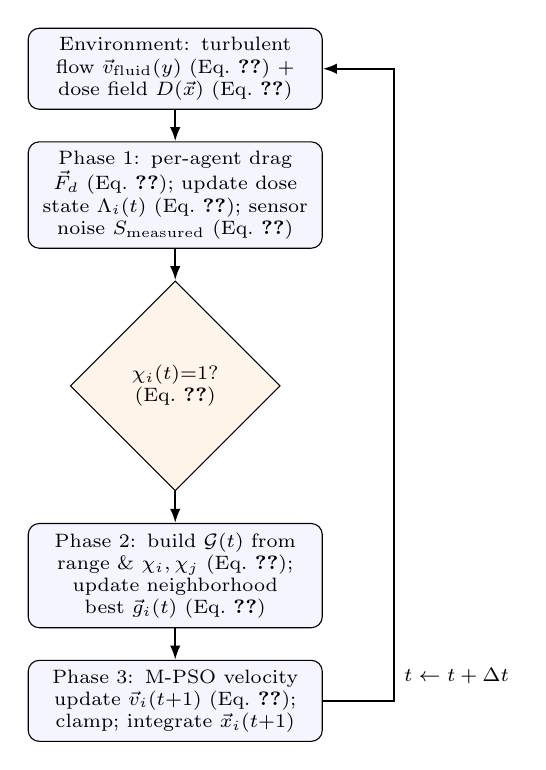
\begin{tikzpicture}[
    node distance=4mm and 4mm,
    box/.style={draw, rounded corners, align=center, minimum height=6.5mm, font=\scriptsize, text width=3.5cm, fill=blue!4},
    decbox/.style={draw, diamond, align=center, font=\scriptsize, fill=orange!8, inner sep=1pt, text width=2.0cm},
    arr/.style={-{Latex[length=1.8mm]}, thick}
]
\node[box] (env) {Environment: turbulent flow $\vec{v}_{\text{fluid}}(y)$ (Eq.~\ref{eq:vfluid}) + dose field $D(\vec{x})$ (Eq.~\ref{eq:dose})};
\node[box, below=of env] (phys) {Phase 1: per-agent drag $\vec{F}_d$ (Eq.~\ref{eq:drag}); update dose state $\Lambda_i(t)$ (Eq.~\ref{eq:cumdose}); sensor noise $S_{\text{measured}}$ (Eq.~\ref{eq:sensor-noise})};
\node[decbox, below=of phys] (chi) {$\chi_i(t){=}1$? (Eq.~\ref{eq:pdrop})};
\node[box, below=of chi] (graph) {Phase 2: build $\mathcal{G}(t)$ from range \& $\chi_i,\chi_j$ (Eq.~\ref{eq:comm-edge}); update neighborhood best $\vec{g}_i(t)$ (Eq.~\ref{eq:local-gbest})};
\node[box, below=of graph] (kin) {Phase 3: M-PSO velocity update $\vec{v}_i(t{+}1)$ (Eq.~\ref{eq:velocity-update}); clamp; integrate $\vec{x}_i(t{+}1)$};
\draw[arr] (env) -- (phys);
\draw[arr] (phys) -- (chi);
\draw[arr] (chi) -- (graph);
\draw[arr] (graph) -- (kin);
\draw[arr] (kin.east) -- ++(0.9,0) |- (env.east) node[pos=0.02, right, font=\scriptsize] {$t \leftarrow t+\Delta t$};
\end{tikzpicture}%
}
\caption{Per-timestep system workflow. A failed channel removes social information but does not halt the physical update.}
\label{fig:blockdiagram}
\end{figure}

\subsection{Kinematic Swarm Update System}
\label{sec:kinematic}

The motion of agent $i \in \{1,\dots,N\}$ is governed by an M-PSO update augmenting the canonical cognitive-social formulation with a physical forcing term from fluid-structure interaction:
\begin{multline}
\vec{v}_i(t+1) = w\,\vec{v}_i(t) + c_1 r_1 \left(\vec{p}_i(t) - \vec{x}_i(t)\right) \\
{} + \chi_i(t)\, c_2 r_2 \left(\vec{g}_i(t) - \vec{x}_i(t)\right) + \frac{\vec{F}_d}{m}\,\Delta t,
\label{eq:velocity-update}
\end{multline}
with forward-Euler position update $\vec{x}_i(t+1) = \vec{x}_i(t) + \vec{v}_i(t+1)\,\Delta t$. The term $(\vec{F}_d/m)\Delta t$ is the principal departure from canonical PSO, embedding Newtonian drag directly into search kinematics. Following PSO convention~\cite{pso_canonical,shi_eberhart_1998}, the cognitive/social terms are an abstract velocity-space input, not a physical force; drag, by contrast, is a genuine kinematic acceleration, explicitly integrated over $\Delta t$ to combine correctly with the algorithmic terms rather than being added as a raw acceleration---precluding agents from executing arbitrarily precise trajectories in a medium that physically resists motion. Eq.~(\ref{eq:velocity-update}) also replaces the canonical global attractor $\vec{g}^{\text{best}}$ with an agent-specific, neighborhood-local attractor $\vec{g}_i(t)$, defined next.

\subsubsection{Dynamic Communication Graph}
\label{sec:comm-graph}

Let $\mathcal{G}(t) = (\mathcal{V}, \mathcal{E}(t))$ denote the swarm communication graph, $\mathcal{V}=\{1,\dots,N\}$. An edge $(j,i)\in\mathcal{E}(t)$---a successful transmission from $j$ to $i$, over a transceiver of fixed physical range $r_{\text{comm}}$---requires joint range and hardware operability:

\begin{equation}
\|\vec{x}_j(t) - \vec{x}_i(t)\| \le r_{\text{comm}} \ \text{and}\ \chi_j(t) = 1 \ \text{and}\ \chi_i(t) = 1,
\label{eq:comm-edge}
\end{equation}
where $\chi_k(t)\sim\text{Bernoulli}(1-P_{\text{drop}}(\vec{x}_k(t)))$ is the per-agent channel state (Sec.~\ref{sec:radiation}), used for both transmit and receive. Thus $\mathcal{N}_i(t)$ collapses to $\{i\}$ when $\chi_i(t)=0$; the explicit social-term gate is a defensive implementation choice, not a separate failure model.

\subsubsection{Neighborhood-Restricted Local Best}
\label{sec:local-best}

The active neighborhood of agent $i$ is $\mathcal{N}_i(t) = \{j \in \mathcal{V} \mid (j,i)\in\mathcal{E}(t)\}\cup\{i\}$, giving a decentralized, neighborhood-specific attractor
\begin{equation}
\vec{g}_i(t) = \arg\max_{j \in \mathcal{N}_i(t)} \left\{ f\left(\vec{p}_j(t)\right) \right\},
\label{eq:local-gbest}
\end{equation}
where $f(\cdot)$ is the noise-corrupted signal fitness. Because $\mathcal{N}_i(t)$ is a stochastic function of $\mathcal{G}(t)$, $\vec{g}_i(t)$ may differ across agents and, in the limit, reduce to full isolation ($\mathcal{N}_i(t)=\{i\}$) when all inbound edges fail simultaneously.

\subsubsection{Notation}
\label{sec:param-defs}

$\vec{x}_i,\vec{v}_i\in\mathbb{R}^2$ are position/velocity; $\vec{p}_i$ and $\vec{g}_i$ are personal and neighborhood-local best states under a maximization fitness $f$; $w,c_1,c_2$ are fixed PSO weights; and $\vec F_d/m$ is drag acceleration. Packet loss is represented only by $\chi_i(t)$, not by changing $c_2$.

\subsection{Turbulent Hydrodynamics and Drag Modeling}
\label{sec:hydro}

Unlike the inert medium assumed by idealized PSO, the PWR coolant pipe presents a fully turbulent flow field that continuously perturbs agent motion. For fully developed flow at Reynolds number $Re>10^5$, the cross-sectional velocity is well-approximated by the empirical one-seventh power-law profile~\cite{turbulent_flow} plus a stochastic fluctuation term:
\begin{equation}
\vec{v}_{\text{fluid}}(y) = v_{\max}\left(1 - \frac{|y|}{R}\right)^{\frac{1}{7}}\hat{i} + \vec{v}_{\text{turb}}, \quad \vec{v}_{\text{turb}} \sim \mathcal{N}(0,\sigma_{\text{turb}}^2),
\label{eq:vfluid}
\end{equation}
where $y\in[-R,R]$ is the wall-normal coordinate, $R$ the pipe radius, $v_{\max}$ the centerline velocity, and $\hat{i}$ the pipe's axial unit vector; the profile enforces no-slip at $y=\pm R$ and a maximum at $y=0$. $\vec{v}_{\text{turb}}$ is a first-order stochastic representation of the Reynolds-decomposed fluctuation $u'=u-\bar{u}$, omitting full RANS closure for tractability while preserving the essential stochastic forcing.

This field couples to agent motion via the standard quadratic drag relation for bluff bodies:
\begin{equation}
\vec{F}_d = -\frac{1}{2}\rho C_d A \left\|\vec{v}_i(t) - \vec{v}_{\text{fluid}}(y)\right\|^2 \hat{u}_d,
\label{eq:drag}
\end{equation}
with $\rho\approx1000\,\text{kg/m}^3$ coolant density, $C_d$ the drag coefficient, $A$ the frontal area, and $\hat{u}_d$ the unit vector opposing relative velocity. This quadratic dependence is strongly non-linear: agents moving against the mean flow near the steep-gradient wall region experience disproportionate resistive forcing, biasing trajectories toward the bulk flow direction---a bias absent from idealized PSO.

\subsection{Ionizing Radiation Degradation Fields}
\label{sec:radiation}

A spatially non-homogeneous gamma field, concentrated near the fissure (corrosion/activation sites co-locate in practice), is modeled as a background term plus inverse-square enhancement:
\begin{equation}
D(\vec{x}) = D_{\text{bg}} + \frac{K}{\|\vec{x}-\vec{x}_f\|^2 + 1.0},
\label{eq:dose}
\end{equation}
with $D_{\text{bg}}$ ambient dose rate, $K$ source intensity, and the $+1.0$ regularizer preventing a singularity at $\vec{x}\to\vec{x}_f$ while permitting severe local dose---an unavoidable mission-success/survivability trade-off, since inspection requires approaching the highest-hazard region.

This drives two mechanistically distinct degradation phenomena~\cite{sensor_degradation}. \textbf{(a) Sensor noise:}
\begin{equation}
S_{\text{measured}}(\vec{x}) = S(\vec{x}) + \epsilon_\gamma, \quad \epsilon_\gamma \sim \mathcal{N}(0,\ \sigma_\gamma^2 D(\vec{x})),
\label{eq:sensor-noise}
\end{equation}
where $S(\vec{x})$ is the true, noise-free proximity signal used as $f(\cdot)$ throughout (peaked at $\vec{x}_f$, decaying with distance), and noise variance scales linearly with dose rate via $\sigma_\gamma^2$, so reliability degrades as agents approach the region of interest. \textbf{(b) Communication loss:}
\begin{equation}
P_{\text{drop}}(\vec{x}) = 1 - e^{-\beta D(\vec{x})},
\label{eq:pdrop}
\end{equation}
with $\beta$ the hardware's dose-to-failure sensitivity ($P_{\text{drop}}\to1$ at high dose; $P_{\text{drop}}\to\beta D(\vec{x})$ at low dose, consistent with a Poisson-thinned first-order failure process). A drop instantaneously zeroes $\chi_i(t)$ (Eq.~\ref{eq:comm-edge}), collapsing Eq.~(\ref{eq:velocity-update}) to purely cognitive-inertial motion for that agent/step---informational isolation, not agent failure, since connectivity may be stochastically restored.

This transient mechanism alone cannot capture \emph{permanent} hardware failure under sustained exposure. Each agent therefore accumulates a running dose state
\begin{equation}
\Lambda_i(t) = \Lambda_i(t-1) + D(\vec{x}_i(t))\,\Delta t, \quad \Lambda_i(0)=0,
\label{eq:cumdose}
\end{equation}
and once $\Lambda_i(t)\ge\Lambda_{\text{fail}}$, the transceiver latches up permanently:
\begin{equation}
\Lambda_i(t) \ge \Lambda_{\text{fail}} \implies \chi_i(t') = 0 \quad \forall\,t'\ge t,
\label{eq:latchup}
\end{equation}
regardless of subsequent position, where $\Lambda_{\text{fail}}$ is a fixed, hardware-specific cumulative-dose failure threshold (Table~\ref{tab:sim-params}). Only Eq.~(\ref{eq:latchup}) is permanent; ordinary Bernoulli drops via $P_{\text{drop}}(\vec{x})$ alone are always transient. It is the swarm's aggregate resilience under this combination of transient isolation and occasional permanent hardware loss---not any individual agent's performance---that is investigated below.

Initial positions are drawn uniformly from $\Omega_{\text{pipe}}=[0,L]\times[-R,R]$; a fixed $v_{\text{clamp}}$ is applied identically to all architectures. The per-timestep phases are the physical/radiological update, graph construction and local-best update, then velocity/position integration (Fig.~\ref{fig:blockdiagram}).

\begin{table}[t]
\renewcommand{\arraystretch}{0.82}
\caption{Simulation configuration. Profiles use $(D_{\text{bg}},K)=(0,0),(0.5,10),(2,100)$.}
\label{tab:sim-params}
\centering\scriptsize\setlength{\tabcolsep}{3pt}
\begin{tabular}{@{}lll@{}}
\toprule Parameter & Symbol & Value \\\midrule
Pipe geometry & $L,R$ & $10.0,1.0$ m \\
Fissure / agent mass & $\vec x_f,m$ & $(8.0,0.9)$ m, $0.05$ kg \\
Flow / turbulence & $v_{\max},\sigma_{\rm turb}$ & $1.5,0.1$ m/s \\
Drag / density & $C_d,A,\rho$ & $0.47,1.26\!\times\!10^{-3}$ m$^2$, 1000 kg/m$^3$ \\
Swarm / horizon & $N,t_{\max}$ & $25,150$ \\
Step / range / clamp & $\Delta t,r_{\rm comm},v_{\rm clamp}$ & $0.1$ s, $2.0$ m, $3.0$ m/s \\
PSO weights & $w,c_1,c_2$ & $0.6,1.2,1.2$ \\
Channel / latch-up & $\beta,\sigma_\gamma,\Lambda_{\rm fail}$ & $0.15$ s/Gy, $0.08$, 300 Gy \\
\bottomrule
\end{tabular}
\end{table}

\section{Simulation Configuration and Results Analysis}
\label{sec:simulation}

The simulator executes $N=25$ agents for 150 steps in a 2D pipe cross-section, with a near-wall fissure at $(8.0,0.9)$ m. Control, Moderate, and Extreme profiles use the three dose-field settings in Table~\ref{tab:sim-params}. A run succeeds if its best estimate comes within 0.3 m of $\vec{x}_f$. All results are generated by \texttt{pso\_nuclear\_sim.py} as independent SHA-256-seeded 500-trial campaigns; velocity clamping is identical across architectures.

\textbf{Choice of $N$ and $t_{\max}$.} The $20\,\text{m}^2$ domain is swept over $N=5$--50 (Table~\ref{tab:sweep-n}); success rises steeply through $N=25$ while cumulative dose and $O(N^2)$ graph cost continue to grow. Thus $N=25$ is an empirical coverage--dose knee, not an a priori choice. $t_{\max}=150$ (15 s) exceeds the observed Control/Moderate plateau and captures the slower Extreme tail.

\begin{figure}[t]
\centering
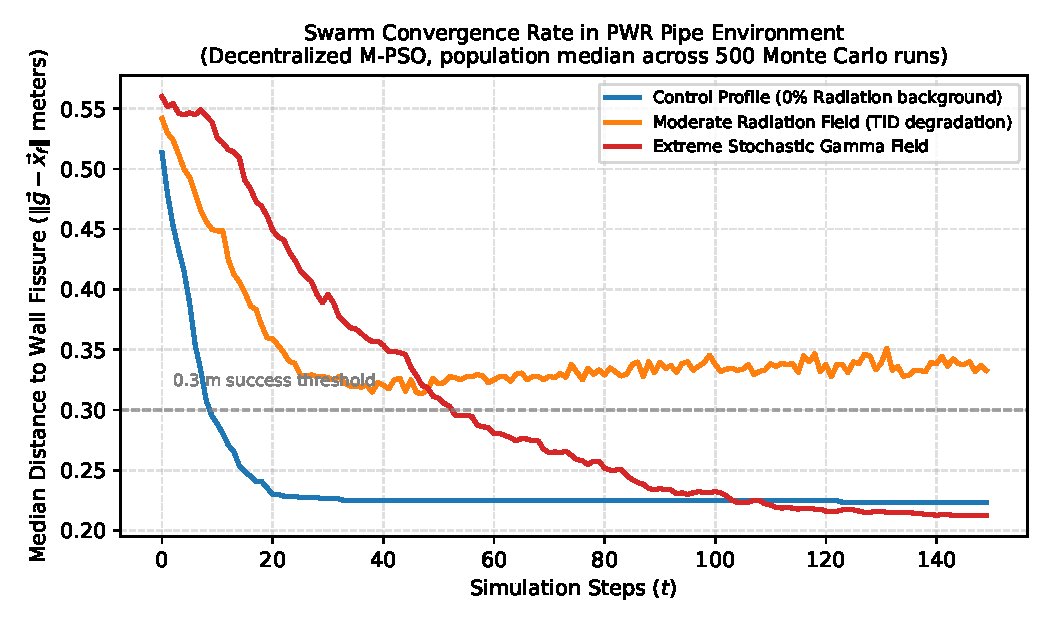
\includegraphics[width=0.84\columnwidth]{pso_convergence_rates.pdf}\\[-1pt]
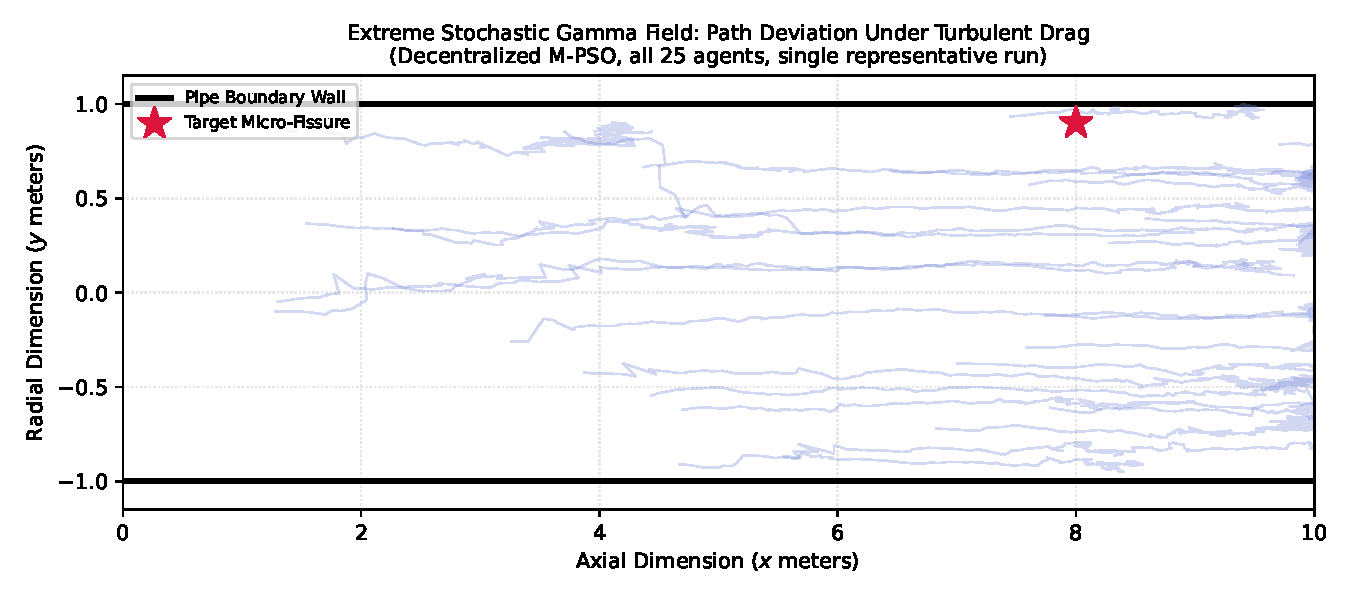
\includegraphics[width=0.84\columnwidth]{pso_swarm_trajectories.pdf}
\caption{Decentralized M-PSO behavior: (top) population-median convergence distance across 500 runs per profile; (bottom) a representative Extreme-profile trajectory realization (25 agents).}
\label{fig:results}
\end{figure}

% Place the only double-column result figure before the table queue.  In
% IEEEtran this avoids a late double-float overtaking Tables III--V.
\begin{figure*}[!t]
\centering
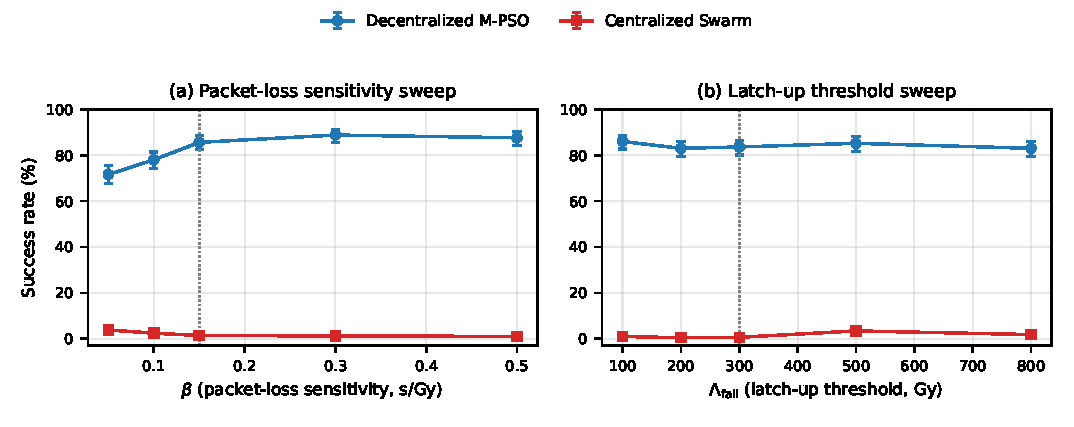
\includegraphics[width=0.93\textwidth]{comm_fragility_sweep.pdf}
\caption{Full communication-fragility campaign (Extreme profile; 500 independent trials per point). Markers show success rate and bars show Wilson 95\% confidence intervals; dotted lines mark the nominal settings. Decentralized M-PSO remains robust to the $\Lambda_{\rm fail}$ sweep, whereas a static leader remains unsuccessful even when hardening greatly reduces leader latch-up.}
\label{fig:fragility-sweep}
\end{figure*}

\subsection{Baseline Comparison}
\label{sec:results}

A Monte Carlo campaign (500 runs/architecture/profile) compares Decentralized M-PSO against two centralized variants and a Canonical PSO. \textbf{Centralized Swarm (static leader):} a single leader broadcasts $\vec{g}^{\text{best}}$, freezing permanently after leader latch-up ($\chi_{\text{leader}}(t)=0$). \textbf{Centralized Swarm (re-election):} an inoperative leader is replaced by the highest-fitness operational, non-latched agent. A post-review hardening check adds one \textbf{hot standby}: the nearest non-leader replicates state only when both radios and range permit, then promotes after $h\in\{1,3,5\}$ consecutive missed heartbeats (timeouts fixed before inspection). These baselines isolate leader dependence through one redundancy level; multi-standby and quorum protocols remain outside scope. \textbf{Canonical PSO:} fully-connected, no drag, no communication-degradation model. Performance is Success Rate (fraction with $\|\vec{g}-\vec{x}_f\|\le0.3\,\text{m}$, with $n_{\text{success}}$ and Wilson-score 95\% CI), Convergence Time, and Cumulative Swarm Dose (Eq.~\ref{eq:cumdose}). Rates also control for trivial spawns: with positions drawn over $\Omega_{\text{pipe}}$ ($\approx20\,\text{m}^2$), an agent can occasionally start within the success radius by chance; non-trivial (search-driven) rates excluding such runs are reported directly in Table~\ref{tab:baseline-comparison} and discussed below.

\begin{table*}[t]
\renewcommand{\arraystretch}{0.85}
\caption{Architecture comparison (500 independent trials per profile/architecture). Values are success [Wilson 95\% CI], non-trivial (search-driven) success, and mean cumulative dose.}
\label{tab:baseline-comparison}
\centering
\scriptsize
\setlength{\tabcolsep}{3pt}
\begin{tabular}{@{}l l c c c c@{}}
\toprule
\textbf{Profile} & \textbf{Architecture} & \textbf{Success (\%) [95\% CI]} & \textbf{$n_{\text{success}}$} & \textbf{Non-triv. (\%)} & \textbf{Cum.\ Dose (Gy)} \\
\midrule
\multirow{4}{*}{Control}
 & Decentralized M-PSO         & 66.0 [61.7,70.0] & 330/500 & 55.6 & $0.0$ \\
 & Centralized (static leader) & 62.0 [57.7,66.1] & 310/500 & 50.4 & $0.0$ \\
 & Centralized (re-election)   & 60.2 [55.8,64.4] & 301/500 & 49.5 & $0.0$ \\
 & Canonical PSO               & 57.0 [52.6,61.3] & 285/500 & 44.3 & $0.0$ \\
\midrule
\multirow{4}{*}{Moderate}
 & Decentralized M-PSO         & 58.0 [53.6,62.2] & 290/500 & 46.3 & $1146.9$ \\
 & Centralized (static leader) & 29.8 [26.0,34.0] & 149/500 & 20.5 & $1387.6$ \\
 & Centralized (re-election)   & \textbf{40.6 [36.4,45.0]} & 203/500 & 31.5 & $1427.6$ \\
 & Canonical PSO               & 42.4 [38.1,46.8] & 212/500 & 24.1 & $3002.4$ \\
\midrule
\multirow{4}{*}{Extreme}
 & Decentralized M-PSO         & \textbf{84.0 [80.5,87.0]} & 420/500 & \textbf{79.9} & $9490.6$ \\
 & Centralized (static leader) & 3.0 [1.8,4.9] & 15/500 & 0.8 & $12610.4$ \\
 & Centralized (re-election)   & 1.8 [0.9,3.4] & 9/500 & 0.8 & $10328.1$ \\
 & Canonical PSO               & 29.6 [25.8,33.7] & 148/500 & 12.9 & $25470.6$ \\
\bottomrule
\end{tabular}

\vspace{2pt}
\raggedright\scriptsize
Each table row is independently SHA-256-seeded; nominally identical settings are independent replications, not shared draws. Four nominal decentralized campaigns span 83.4--87.0\%, with overlapping Wilson CIs, providing an internal stability check.
\end{table*}

\textbf{Control and Moderate.} In Control, all architectures have overlapping CIs (57.0--66.0\%); residual failures are consistent with PSO stagnation once personal and neighborhood best states coincide~\cite{van_den_bergh_2002}. Moderate radiation reduces decentralized success to 58.0\% while the static leader falls to 29.8\%. Re-election partially recovers to 40.6\% because communication remains sufficiently available for the election step.

\textbf{Extreme.} Decentralized M-PSO reaches 84.0\% [80.5,87.0], versus 3.0\% and 1.8\% [0.9,3.4] for the static and re-election baselines. Canonical PSO reaches 29.6\% but omits the modeled communication hazard. In the independent hardening campaign, decentralized success is 87.0\% [83.8,89.7], while all hot-standby variants remain near zero (Table~\ref{tab:hot-standby}). Failover completes in 78.6--81.2\% of trials, so the low success is not an inert-failover artifact. Promotion changes the coordinator, not the information path: reporting and replication use the same range/$\chi$ graph, and both coordinator agents accrue dose. Within the evaluated architectures, one backup therefore does not restore edges lost under Extreme fragmentation.

\begin{table}[t]
\renewcommand{\arraystretch}{0.85}
\caption{Full Ablation Isolation (Extreme Profile, $N=25$, $r_{\text{comm}}=2.0\,\text{m}$; 500-Trial Monte Carlo Campaign per Cell, SHA-256-Seeded per Condition Identity)}
\label{tab:ablation}
\centering
\scriptsize
\setlength{\tabcolsep}{3pt}
\begin{tabular}{@{}p{0.5\columnwidth} c c@{}}
\toprule
\textbf{Configuration} & \textbf{Success (\%) [95\% CI]} & \textbf{Non-triv.\ (\%)} \\
\midrule
A. Full M-PSO model (drag, explicit $\chi$-gate, both degradation channels) & 84.4 [81.0, 87.3] & 79.9 \\
B. No drag term & 23.8 [20.3, 27.7] & 0.0 \\
C. No communication degradation ($\chi_i(t)\!\equiv\!1$; fully connected, no latch-up) & 44.8 [40.5, 49.2] & 30.9 \\
D. Canonical PSO $+$ drag (non-decentralized) & 38.0 [33.9, 42.3] & 26.4 \\
E. No explicit $\chi$-gate (self-collapse of $\mathcal{N}_i(t)$ only) & 83.8 [80.3, 86.8] & 79.0 \\
F. Sensor-noise only (no packet loss; latch-up still active) & 41.8 [37.6, 46.2] & 28.0 \\
G. Packet-loss only (no sensor noise) & 93.2 [90.6, 95.1] & 91.3 \\
\bottomrule
\end{tabular}

\vspace{2pt}
\raggedright\scriptsize
Cell A replicates the nominal Table~\ref{tab:baseline-comparison} configuration independently (see footnote a there). Cells E vs.\ A isolate the explicit $\chi_i(t)$ social-term gate: $83.8\%$ vs.\ $84.4\%$, CIs almost fully overlapping---the gate offers only a marginal benefit over neighborhood self-collapse alone (Sec.~\ref{sec:comm-graph}). Cell D vs.\ the Canonical PSO row of Table~\ref{tab:baseline-comparison} ($29.6\%$) isolates drag's main effect independent of topology: $38.0\%$ [33.9, 42.3] is a modest but real $+8.4$-point improvement over the drag-free canonical baseline (CIs only marginally overlapping, at $33.7$--$33.9\%$). This is far smaller than drag's effect within the decentralized architecture (cf.\ A vs.\ B, $84.4\%$ vs.\ $23.8\%$, a $+60.6$-point gain), indicating a strong positive interaction between drag-awareness and decentralized topology rather than an architecture-independent main effect alone.\textsuperscript{d}\\[2pt]
\textsuperscript{d}Corrected value. An earlier version of the simulator's drag-application logic evaluated \texttt{architecture=="Canonical PSO" or not use\_drag} as a single boolean gate, which unconditionally skipped drag for the Canonical PSO architecture regardless of the \texttt{use\_drag} flag. This silently defeated cell D's intended configuration (drag genuinely enabled on a non-decentralized architecture); the previously reported $26.6\%$ [22.9, 30.6] reflected two independently-seeded \emph{drag-free} Canonical PSO runs, not a drag-vs-no-drag comparison. The bug is fixed in the released simulator (Sec.~\ref{sec:avail}) by making drag application depend solely on \texttt{use\_drag}, independent of architecture; $38.0\%$ above is the corrected, re-run result under the same $n{=}500$ trial count and condition identity.
\end{table}

\textbf{Ablation isolation.} Table~\ref{tab:ablation} isolates drag-awareness, the explicit $\chi_i(t)$ social-term gate, and the two radiological channels, across all seven configurations (Extreme profile). Removing drag alone (cell B) collapses Decentralized M-PSO to $23.8\%$, with \emph{zero} non-trivial success---without drag compensation, agents cannot meaningfully navigate the turbulent flow. Adding drag to the non-decentralized Canonical PSO architecture (cell D) yields $38.0\%$ [33.9, 42.3]\textsuperscript{d}---a modest $+8.4$-point improvement over the drag-free Canonical baseline ($29.6\%$, Table~\ref{tab:baseline-comparison})---while disabling communication degradation entirely (cell C) reaches $44.8\%$. Drag therefore has a real but modest architecture-independent effect, and a much larger effect with decentralized topology (A vs.\ B: $+60.6$ points). The corresponding difference-in-differences interaction is $52.2$ points (Wald $z=13.4$, $p<10^{-40}$; 95\% CI $[44.6,59.8]$ points), supporting an interaction rather than a decentralization-exclusive drag effect. The explicit $\chi_i(t)$ social-term gate is not load-bearing: cell E gives $83.8\%$ [80.3,86.8], within noise of cell A's $84.4\%$. The radiological channels are non-additive: sensor noise alone is harmful ($41.8\%$, F), while packet-loss only gives $93.2\%$ (466/500, G) versus $84.4\%$ (422/500, A), an $8.8$-point difference (two-sided two-proportion $z=4.4$, $p<10^{-4}$; 95\% difference CI $[4.9,12.7]$ points). In this reduced-order model, fragmentation without noisy fitness signals behaves as a diversity mechanism; it is not a recommendation to increase packet loss in deployed systems.

Taken together, these results show a large architecture-dependent advantage under the modeled Extreme profile: relative to the evaluated static-leader and re-election baselines, decentralized M-PSO reaches $84.0\%$ versus $3.0\%$ and $1.8\%$. This comparison isolates the vulnerability of leader dependence under coupled radiation and communication degradation; it does not establish that every possible fault-tolerant centralized design would fail.

\subsection{Sensitivity to Swarm Size and Communication Range}
\label{sec:sensitivity}

The results above fix $N=25$ and $r_{\text{comm}}=2.0\,\text{m}$ (Table~\ref{tab:sim-params}). To characterize robustness and generalization beyond the noise/radiation axis already varied across profiles, two further Monte Carlo sweeps (500 trials per condition, Extreme profile, identical success threshold) vary these system parameters directly.

\begin{table}[t]
\renewcommand{\arraystretch}{0.85}
\caption{Swarm-size sensitivity (Extreme profile; 500 independent trials per $N$).}
\label{tab:sweep-n}
\centering
\scriptsize
\setlength{\tabcolsep}{3pt}
\begin{tabular}{@{}c c c c c@{}}
\toprule
$N$ & Success (\%) & 95\% CI & Mean Conv.\ (steps) & Cum.\ Dose (Gy) \\
\midrule
10 & 59.4 & [55.0, 63.6] & 49.8 & 3717.1 \\
\textbf{25} & \textbf{83.4} & \textbf{[79.9, 86.4]} & \textbf{30.6} & \textbf{9489.6} \\
50 & 98.8 & [97.4, 99.4] & 17.0 & 19208.9 \\
\bottomrule
\end{tabular}

\end{table}

\textbf{Swarm size.} Table~\ref{tab:sweep-n} shows the coverage--dose trade-off: performance rises steeply through $N=25$, while dose grows linearly. Larger swarms improve success but duplicate coverage and increase exposure, motivating the selected knee.

\begin{table}[t]
\renewcommand{\arraystretch}{0.84}
\caption{Communication-fragility sensitivity (Extreme profile; 500 independent trials per row). Success is [Wilson 95\% CI]. $D$: decentralized; $C$: static leader.}
\label{tab:fragility}
\centering\scriptsize\setlength{\tabcolsep}{3pt}
\begin{tabular}{@{}lccc@{}}
\toprule Setting & $D$ success & $C$ success & $C$ latch-up \\\midrule
$\beta=0.05$ s/Gy & 71.6 [67.5,75.4] & 3.8 [2.4,5.9] & 92.8\% \\
$\beta=0.50$ s/Gy & 87.6 [84.4,90.2] & 1.0 [0.4,2.3] & 52.6\% \\
$\Lambda_{\rm fail}=100$ Gy & 86.0 [82.7,88.8] & 1.0 [0.4,2.3] & 100.0\% \\
$\Lambda_{\rm fail}=800$ Gy & 83.0 [79.5,86.0] & 1.8 [0.9,3.4] & 9.4\% \\
\bottomrule
\end{tabular}
\end{table}

\begin{table}[t]
\renewcommand{\arraystretch}{0.84}
\caption{Single-hot-standby robustness (Extreme; 500 trials/$h$). Success: [Wilson 95\% CI]; non-triv.: \% (successes/eligible starts).}
\label{tab:hot-standby}
\centering\scriptsize\setlength{\tabcolsep}{2.5pt}
\begin{tabular}{@{}cccc@{}}
\toprule
$h$ & Success (\%) [95\% CI] & Failover (\%) & Non-triv. (\%) \\
\midrule
1 & 1.4 [0.7,2.9] & 81.2 & 0.26 (1/391) \\
3 & 1.6 [0.8,3.1] & 80.4 & 0.00 (0/392) \\
5 & 0.6 [0.2,1.7] & 78.6 & 0.00 (0/393) \\
\bottomrule
\end{tabular}
\end{table}

\textbf{Neighbor and channel failure dynamics.} Eq.~\ref{eq:comm-edge} applies to every transceiver, not only a leader. The original range sweep left decentralized success within 80.4--87.0\% over $r_{\rm comm}=0.5$--3.0 m, while the static leader remained 0.6--2.4\%. Table~\ref{tab:fragility} adds hardware/channel sensitivity: decentralized performance remains 83.0--86.0\% across $\Lambda_{\rm fail}=100$--800 Gy, whereas hardening the leader lowers its latch-up incidence without restoring centralized success. The $\beta$ trend is a model-specific observation, not a recommendation to increase packet loss.

\textbf{Relation to learning-based coordination.} QMIX and MAPPO are relevant centralized-training/decentralized-execution baselines for cooperative control~\cite{rashid_qmix_2018,yu_mappo_2022}. They are not assigned numerical results here: a defensible comparison requires the same local observations, hazard process, training budget, and held-out degradation shifts. In contrast, the present M-PSO controller is training-free and exposes its dose and communication gates explicitly; Fig.~\ref{fig:fragility-sweep} therefore establishes robustness only for this model, rather than claiming superiority over learned policies.

\section{Conclusion and Future Work}
\label{sec:conclusion}

This paper presents a reproducible computational framework for fault-tolerant, drag-aware swarm control under radiation-driven sensing and communication degradation. Under the modeled Extreme profile, decentralized M-PSO attains 84.0\% success versus 3.0\% for a static leader and 1.8\% after leader re-election; a separate hot-standby campaign remains at 0.6--1.6\% across three pre-specified timeouts despite frequent failover activation. The targeted ablation shows that drag has a modest architecture-independent effect but a much larger effect when combined with decentralized topology. The channel, latch-up, and standby studies sharpen the bounded conclusion: among the leader-based architectures evaluated here, neither transceiver hardening nor one replicated backup resolves the vulnerability induced by a privileged coordination point.

\textbf{Limitations and future work:} The model is 2D and uses a one-seventh-power-law flow approximation, homogeneous agents, and no thermal-hydraulic coupling or hardware validation. $N$, $r_{\rm comm}$, $\beta$, and $\Lambda_{\rm fail}$ are swept, but $(w,c_1,c_2)$ remain illustrative; one hot standby does not exhaust multi-backup or quorum-based centralized protocols. Future work includes matched MARL experiments, multi-standby/majority consensus, 3D CFD, relay heterogeneity, and flow-loop validation.

\section*{Code and Data Availability}
\label{sec:avail}
The simulator, campaign scripts, seed policy, tests, and result summaries are released with this manuscript at \url{https://doi.org/10.5281/zenodo.22166217}. Every campaign uses collision-proof SHA-256 condition-identity, per-trial seeding. The release documents the corrected Canonical-PSO drag ablation and includes the seven-cell ablation, re-election, communication-fragility, and hot-standby campaigns.

% Tighten bibliography inter-item spacing and font (safe IEEEtran patch, no content change)
\let\OLDthebibliography\thebibliography
\renewcommand\thebibliography[1]{%
  \OLDthebibliography{#1}%
  \scriptsize
  \setlength{\itemsep}{0pt}%
  \setlength{\parskip}{0pt}%
}

\bibliographystyle{IEEEtran}
\bibliography{references_IECON}

\end{document}
